% ============================================================
% CTU Journal of Science — LaTeX Template
% Tạp chí Khoa học Đại học Cần Thơ
% Phần A: Khoa học Tự nhiên, Công nghệ và Môi trường
%
% Định dạng chuẩn xuất bản: Khổ A4, 2 cột (body), 1 cột (title/authors)
% Lề: top/bottom=2.5cm, left/right=1.8cm, columnsep=0.8cm
% Spacing: Single spacing, Font size: 10pt
% ============================================================

\documentclass[10pt, a4paper, twocolumn]{article}

% ── Encoding & Language ─────────────────────────────────────
\usepackage[utf8]{inputenc}
\usepackage[T5]{fontenc}          % Vietnamese encoding
\usepackage[english,vietnamese]{babel} % vietnamese is active language
\usepackage{times}                % Times New Roman equivalent

% ── Page Layout ─────────────────────────────────────────────
\usepackage[
  top=2.5cm, bottom=2.5cm,
  left=1.8cm, right=1.8cm,
  columnsep=0.8cm
]{geometry}
\usepackage{setspace}
\singlespacing                    % Bản in chính thức dùng single-spaced
% \raggedbottom removed — cho phép so le nhẹ giữa 2 cột (flushbottom mặc định)

% ── Mathematics ─────────────────────────────────────────────
\usepackage{amsmath}
\usepackage{amssymb}
\usepackage{mathtools}

% ── Figures & Tables ────────────────────────────────────────
\usepackage{graphicx}
\usepackage{booktabs}
\usepackage{longtable}
\usepackage{multirow}
\usepackage{array}
\usepackage{tabularx}
\usepackage{dblfloatfix}   % thay stfloats, cho phép figure*/table* dùng [b]
\usepackage{caption}
\usepackage{placeins}
\usepackage{cuted}
\usepackage{needspace}
\usepackage{adjustbox}
\usepackage{caption}
\usepackage{tikz}
\usetikzlibrary{positioning, shapes.geometric}

% ── Section Formatting (CTU Style) ──────────────────────────
\usepackage{titlesec}
\titleformat{\section}{\large\bfseries}{\thesection.}{0.5em}{\MakeUppercase}
\titleformat{\subsection}{\normalsize\bfseries}{\thesubsection.}{0.5em}{}
\titleformat{\subsubsection}{\normalsize\itshape}{\thesubsubsection.}{0.5em}{}

% ── Float Control (Dense Packing) ───────────────────────────
\renewcommand{\topfraction}{0.95}
\renewcommand{\bottomfraction}{0.95}
\renewcommand{\floatpagefraction}{0.85}
\renewcommand{\textfraction}{0.05}
\renewcommand{\dbltopfraction}{0.95}
\renewcommand{\dblfloatpagefraction}{0.85}

% Caption format: Bold, no period
% Table caption: above, left-aligned
% Figure caption: below, centered
\captionsetup[table]{
  labelfont=bf, textfont=bf,
  justification=raggedright,
  singlelinecheck=false,
  position=above,
  labelsep=period,
  font=small
}
\captionsetup[figure]{
  labelfont=bf, textfont=bf,
  justification=centering,
  position=below,
  labelsep=period,
  font=small
}

% ── Hyperlinks & References ──────────────────────────────────
\usepackage[
  hidelinks,
  colorlinks=false
]{hyperref}
\usepackage{url}

% APA-style bibliography (author-year)
\usepackage[
  backend=biber,
  style=authoryear,
  sorting=nyt,            % Sort by name, year, title
  natbib=true
]{biblatex}
\addbibresource{references.bib}
\DeclareLanguageMapping{vietnamese}{english}

\DefineBibliographyStrings{vietnamese}{
  andothers = {và cs\adddot},
  and = {và},
  in = {trong},
  inproceedings = {trong Kỷ yếu},
  incollection = {trong Tuyển tập},
  inbook = {trong Sách},
  journal = {Tạp chí},
  volume = {tập},
  number = {số},
  pages = {tr\adddot},
  page = {tr\adddot},
  techreport = {Báo cáo kỹ thuật},
  editor = {chủ biên},
  editors = {chủ biên},
  edition = {tái bản},
  url = {URL},
  note = {Ghi chú},
  doi = {DOI},
  isbn = {ISBN},
  issn = {ISSN},
  phdthesis = {Luận án Tiến sĩ},
  mastersthesis = {Luận văn Thạc sĩ},
}
\renewcommand{\intitlepunct}{\addspace}

% ── Section formatting (CTU style) ──────────────────────────
\usepackage{titlesec}
% Level 1: UPPERCASE, BOLD, numbered
\titleformat{\section}
  {\normalfont\normalsize\bfseries\MakeUppercase}
  {\thesection.}{0.5em}{}
% Level 2: Title Case, Bold
\titleformat{\subsection}
  {\normalfont\normalsize\bfseries}
  {\thesubsection.}{0.5em}{}
% Level 3: Italic, Title Case
\titleformat{\subsubsection}
  {\normalfont\normalsize\itshape}
  {\thesubsubsection.}{0.5em}{}

% ── Running Headers & Footers (CTU Style) ────────────────────
\usepackage{fancyhdr}
\pagestyle{fancy}
\fancyhf{}
\fancyhead[LO,RE]{\small\itshape Tạp chí Khoa học Đại học Cần Thơ}
\fancyhead[RO,LE]{\small\itshape Tập ..., Số ... (...): ...-...}
\fancyfoot[C]{\thepage}
\renewcommand{\headrulewidth}{0.4pt}

% ── Miscellaneous ────────────────────────────────────────────
\usepackage{xcolor}
\usepackage{enumitem}
\usepackage{microtype}
\usepackage{float}
\usepackage{subcaption}
\usepackage{authblk}

% ============================================================
% DOCUMENT BEGINS
% ============================================================
\begin{document}

% ── Title and Authors in Single Column at the top of Page 1 ──
\twocolumn[{
  \noindent\small\textit{Tạp chí Khoa học Đại học Cần Thơ} \hfill \textit{Tập ..., Số ... (...): ...-...}\\
  \noindent\rule{\textwidth}{0.5pt}
  \vspace{0.8em}
  
  \begin{center}
    {\large\bfseries
      PHÁT HIỆN THỂ CHẾ VÀ GIẢI THÍCH GIÁ ĐIỆN PHI TUYẾN TẠI SÁU THỊ TRƯỜNG CHÂU ÂU GIAI ĐOẠN 2018--2025
    }\\[0.8em]

    {\large\bfseries
      ELECTRICITY MARKET REGIME DISCOVERY AND NONLINEAR PRICE EXPLANATION FROM SIX EUROPEAN MARKETS, 2018--2025
    }\\[1.2em]

    {\normalsize\itshape
      Tác giả\textsuperscript{1*}\\[0.2em]
      \textsuperscript{1}Trường Công nghệ thông tin \& Truyền thông, Đại học Cần Thơ, Việt Nam\\[0.2em]
      *Email: tacgia@ctu.edu.vn
    }\\[1.5em]
  \end{center}
}]
\thispagestyle{empty}

% ── Left Column: Article Information ─────────────────────────
\subsection*{Thông tin chung\\(Article Information)}
\noindent\rule{\columnwidth}{0.4pt}
\vspace{0.5em}
{\small
\textbf{Nhận bài (Received):} .../.../...\\
\textbf{Sửa bài (Revised):} .../.../...\\
\textbf{Duyệt đăng (Accepted):} .../.../...\\
\vspace{1em}

\noindent\textbf{Title:}\\
ELECTRICITY MARKET REGIME DISCOVERY AND NONLINEAR PRICE EXPLANATION FROM SIX EUROPEAN MARKETS, 2018--2025\\
\vspace{1em}

\noindent\textbf{Author(s):}\\
Tác giả\\
\vspace{1em}

\noindent\textbf{Affiliation(s):}\\
\textsuperscript{1}College of Information and Communication Technology, Can Tho University, Vietnam\\
\vspace{1em}

\noindent\textbf{*Corresponding author:}\\
Email: tacgia@ctu.edu.vn
}

% ── Switch to Right Column for Abstracts ─────────────────────
\newpage

% ── Right Column: Bilingual Abstracts ────────────────────────
\noindent\textbf{TÓM TẮT}\\
\textit{\small
  Nghiên cứu này điều tra cơ chế nhân quả liên kết nền tảng vật lý với giá điện bán buôn tại sáu thị trường châu Âu (2018--2025). Chúng tôi đề xuất quy trình bốn giai đoạn: (i) kiểm định Granger xác nhận chuỗi Merit Order, (ii) mô hình OLS xác định phi tuyến cấu trúc, (iii) phát hiện thể chế thị trường qua UMAP và HDBSCAN, (iv) XGBoost và phân rã SHAP giải thích giá phi tuyến. Phân rã STL cho thấy khủng hoảng 2022 nằm chủ yếu trong phần dư, độc lập với xu hướng và mùa vụ. Kết quả phát hiện từ 5 đến 10 thể chế thị trường phi tham số. Kiểm định cửa sổ mở rộng dần (walk-forward) xác nhận dịch chuyển phân phối nghiêm trọng năm 2022 ($R^2 < 0$) và phục hồi năm 2023. Phân tích SHAP chứng minh giá khí TTF và tải trọng còn lại là yếu tố chi phối; nhãn thể chế cung cấp giá trị diễn giải nhưng không cải thiện đáng kể độ chính xác dự báo ($\Delta R^2 \approx +0{,}012$).
}\\[0.4em]
\noindent\textit{\small\textbf{Từ khóa:} dự báo giá điện, HDBSCAN, Merit Order, thể chế thị trường, SHAP, UMAP, XGBoost}
\vspace{1.0em}

\noindent\textbf{ABSTRACT}\\
\textit{\small
  This paper investigates the causal mechanism linking physical fundamentals to wholesale electricity prices across six European markets (2018--2025). We propose a four-stage pipeline: (i) Granger causality validation of the Merit Order, (ii) OLS linear benchmarking for structural nonlinearities, (iii) unsupervised market regime discovery via UMAP and HDBSCAN, and (iv) walk-forward XGBoost with SHAP for nonlinear price explanation. STL decomposition reveals the 2022 crisis is embedded in the residual component, unexplainable by trend or seasonality. Regime discovery identifies 5--10 structurally distinct market states per country. Walk-forward validation confirms severe distribution shift in 2022 ($R^2 < 0$) followed by strong recovery in 2023. SHAP analysis reveals TTF gas price and residual load as dominant drivers; regime labels provide interpretable market-state descriptions but contribute negligible predictive accuracy improvement ($\Delta R^2 \approx +0.012$).
}\\[0.4em]
\noindent\textit{\small\textbf{Keywords:} electricity price forecasting, HDBSCAN, market regime, Merit Order, SHAP, UMAP, XGBoost}



% ── Page Break to Start Main Text on Page 2 ──────────────────
\newpage

% ============================================================
% sections/introduction.tex
% Section 1: GIỚI THIỆU

\section{Giới thiệu}

Thị trường bán buôn điện châu Âu đã trải qua thời kỳ biến động chưa từng có trong giai đoạn 2021--2022 \citep{iea2022}. Tại sáu quốc gia Trung và Tây Âu được nghiên cứu, bao gồm Đức (DE), Đan Mạch (DK), Tây Ban Nha (ES), Pháp (FR), Ý (IT) và Ba Lan (PL), giá điện bán buôn vốn duy trì ổn định trong khoảng 40--80 EUR/MWh giai đoạn 2018--2020 đã tăng vọt tới mức kỷ lục vượt quá 500 EUR/MWh trong các đợt cao điểm của cuộc khủng hoảng năng lượng. Các mô hình kinh tế lượng tuyến tính truyền thống, được hiệu chuẩn dựa trên dữ liệu trước khủng hoảng, hầu như thất bại trong việc giải thích hành vi giá bất thường này, với sai số tuyệt đối trung bình (MAE) vượt quá 100 EUR/MWh trong giai đoạn cao điểm khủng hoảng \citep{lago2021}.

Câu hỏi nghiên cứu cốt lõi thúc đẩy nghiên cứu này là: \textit{Chuỗi nhân quả Merit Order (vận hành từ sản lượng nguồn năng lượng tái tạo và phụ tải hệ thống để xác định tải trọng còn lại, kết hợp với chi phí nhiên liệu đầu vào để hình thành giá điện) vận hành như thế nào trong điều kiện bình thường, và cơ chế nào đã khuếch đại chuỗi này thành một cuộc khủng hoảng giá điện?}

Nguyên lý Merit Order quy định rằng giá thị trường điện được quyết định bởi chi phí cận biên của nhà máy điện đắt nhất được huy động để đáp ứng nhu cầu \citep{sensfuss2008}. Trong điều kiện bình thường, nguồn phát năng lượng tái tạo dồi dào sẽ giảm tải trọng còn lại (Residual Load) cần đáp ứng bởi các nguồn phát nhiên liệu hóa thạch, từ đó giảm xác suất các nhà máy khí đốt đắt đỏ trở thành đơn vị cận biên thiết lập giá. Tuy nhiên, trong cuộc khủng hoảng 2021--2022, sự kết hợp đồng thời của điều kiện gió yếu, sản lượng điện hạt nhân sụt giảm nghiêm trọng tại Pháp và cú sốc nguồn cung khí đốt toàn cầu đã làm sụp đổ hoàn toàn cơ chế tự ổn định này \citep{iea2022}.

Các nghiên cứu hiện tại thường sử dụng mô hình chuyển đổi thể chế có tham số (regime-switching models) như trong nghiên cứu của \citet{janczura2010} và \citet{huisman2003}, vốn đòi hỏi các giả định phân phối khắt khe và không phù hợp với đặc tính phân phối đuôi dày (heavy-tailed distribution) của giá điện. Nghiên cứu này đóng góp một khung phân tích hoàn toàn phi tham số, kết hợp UMAP \citep{mcinnes2018} và HDBSCAN \citep{campello2013} để phát hiện các thể chế thị trường một cách tự động, sau đó áp dụng thuật toán XGBoost \citep{chen2016} cùng với phân rã SHAP \citep{lundberg2017} để định lượng phi tuyến đóng góp của từng nhân tố. Phương pháp này mang lại các kết quả có tính nhất quán cao và khả năng tái lập trên sáu thị trường có cấu trúc nguồn phát khác nhau.

Các đóng góp chính của nghiên cứu này bao gồm:
\begin{enumerate}[label=(\roman*)]
  \item Đề xuất quy trình phát hiện thể chế thị trường điện phi tham số, không phụ thuộc giả định phân phối và loại bỏ hoàn toàn hiện tượng rò rỉ dữ liệu mục tiêu (target leakage).
  \item Cung cấp bằng chứng thực nghiệm chéo từ sáu quốc gia đại diện cho các cấu trúc năng lượng khác nhau, trải qua ba giai đoạn kinh tế (trước khủng hoảng, khủng hoảng và sau khủng hoảng).
  \item Định lượng độ nhạy cảm của giá điện đối với các nhân tố đầu vào theo từng thể chế thông qua phân rã SHAP theo cơ chế kiểm chứng cửa sổ mở rộng dần (Walk-Forward Expanding Window).
  \item Xác định ranh giới khủng hoảng phi tuyến thực nghiệm trong không gian sáu biến trạng thái (Tải trọng còn lại, Giá khí TTF, Giá than, Giá tín chỉ EU ETS, Giá dầu Brent, Độ lệch trữ lượng khí).
\end{enumerate}

% ============================================================


% ============================================================
% sections/methodology.tex
% Section 2: PHƯƠNG PHÁP NGHIÊN CỨU

\section{Phương pháp nghiên cứu}

\subsection{Dữ liệu và phân rã chuỗi thời gian}

Nghiên cứu sử dụng tập dữ liệu quy mô lớn gồm 420.768 quan sát theo giờ từ sáu quốc gia châu Âu giai đoạn 2018--2025: Đức (DE), Đan Mạch (DK), Tây Ban Nha (ES), Pháp (FR), Ý (IT) và Ba Lan (PL). Bộ dữ liệu gốc bao phủ 17 quốc gia châu Âu; sáu quốc gia trên được lựa chọn từ tập hợp này theo năm tiêu chí đồng thời nhằm tối đa hóa tính đại diện về mặt phương pháp luận: (1)~\textit{Cơ cấu nguồn phát đa dạng}, trong đó mỗi quốc gia đại diện cho ít nhất một dạng nguồn phát chính trong hệ thống Merit Order; (2)~\textit{Phủ toàn phổ Tải trọng còn lại (Residual Load)}, bao gồm từ giá âm do dư thừa tái tạo (DK) đến giá bùng nổ do thiếu nguồn cung (IT); (3)~\textit{Đa dạng địa lý}, phủ kín năm vùng khí hậu của châu Âu (Bắc, Trung, Tây, Đông, Nam); (4)~\textit{Mức độ độc lập thị trường}, ưu tiên các thị trường có giá phản ánh cơ chế nội tại, không bị chi phối bởi dòng nhập khẩu qua đường dây liên kết; và (5)~\textit{Khả năng kiểm chứng chuỗi nhân quả}, trong đó mỗi quốc gia phải thể hiện rõ ít nhất một mắt xích trong chuỗi Merit Order.

Sự kết hợp của sáu quốc gia đảm bảo bao phủ đầy đủ năm loại nguồn phát chính trong hệ thống châu Âu: DE (cơ cấu hỗn hợp gió--than--khí đang chuyển đổi), DK (gió ngoài khơi chiếm hơn 50\% sản lượng), ES (năng lượng mặt trời cao cùng cơ chế áp trần giá khí đốt phát điện tạo ra sự cô lập tương đối với thị trường khí đốt EU), FR (điện hạt nhân chi phối $\approx$70\% và sự sụt giảm sản lượng năm 2022 làm mất nguồn phát nền cố định baseload), IT (quốc gia phụ thuộc khí đốt nhập khẩu nhiều nhất trong EU, nơi quá trình truyền dẫn từ giá TTF sang giá điện diễn ra mạnh nhất), và PL (nhiệt điện than chi phối $\approx$70\%, là phép thử cho trường hợp Merit Order thuần nhiên liệu hóa thạch không bị can nhiễu bởi tái tạo). Mười một quốc gia còn lại bị loại theo ba nhóm lý do có cơ sở phương pháp luận rõ ràng: (i)~\textit{Thủy điện hồ chứa điều phối được chi phối} (Na Uy, Thụy Điển, Áo, Thụy Sĩ). Cụ thể, trong hệ thống Merit Order, giá điện được quyết định bởi chi phí của nhà máy \textit{cuối cùng} (đắt nhất) được huy động để đáp ứng nhu cầu, gọi là \textit{nhà máy cận biên quyết định giá} (marginal plant), và giá của nó trở thành giá thị trường cho tất cả nhà máy đang vận hành. Tại Na Uy và Thụy Điển, nơi thủy điện hồ chứa điều phối được chiếm tới 70--90\% sản lượng, nhà vận hành chủ động mở thêm cửa xả turbine khi cầu tăng, khiến thủy điện tự lấp đầy khoảng trống trước khi nhà máy than hay khí, vốn có chi phí cao hơn nhiều, cần được huy động. Do đó, nhà máy nhiên liệu hóa thạch gần như không bao giờ trở thành nhà máy đắt nhất quyết định giá. Thay vào đó, giá điện phụ thuộc vào \textit{giá trị kinh tế cận biên của thủy điện hồ chứa} (Water Value), tức chi phí cơ hội giữa việc xả nước phát điện tại thời điểm hiện tại so với việc tích trữ cho giai đoạn giá cao hơn. Đây là cơ chế định giá hoàn toàn nằm ngoài khung Merit Order nhiên liệu hóa thạch mà nghiên cứu này kiểm chứng. (ii)~\textit{Thị trường không đủ độc lập} (Bỉ, Hà Lan, Ireland): giá bị chi phối chủ yếu bởi dòng nhập khẩu qua đường dây liên kết xuyên biên giới. (iii)~\textit{Trùng lặp vai trò đại diện} (Séc, Slovakia, Hungary, Phần Lan). Lưu ý rằng \textit{Hydro\_RoR\_MW} (lòng sông, không điều phối được) và \textit{Hydro\_Reservoir\_MW} (hồ chứa) vẫn được đưa vào tập đặc trưng của sáu quốc gia được chọn vì tại các thị trường này thủy điện chỉ chiếm 5--15\% sản lượng và nhiên liệu hóa thạch vẫn là nguồn phát cận biên quyết định giá, điều này hoàn toàn nhất quán với lý do loại bỏ các thị trường thủy điện chi phối.

Biến mục tiêu là giá bán buôn điện thực tế đã điều chỉnh lạm phát theo chỉ số giá tiêu dùng HICP (HICP-adjusted Real Wholesale Price, ký hiệu là \textit{Real\_Wholesale\_Price\_EUR}). Các biến giải thích vật lý và kinh tế vĩ mô được thu thập từ ENTSO-E, EMBER, ICE, EEX và GIE AGSI+.

Để hiểu rõ đặc tính chuyển dịch cấu trúc của giá điện trước khi đi vào phân tích nhân quả phức tạp, chúng tôi áp dụng phương pháp phân rã xu hướng và mùa vụ STL (Seasonal-Trend decomposition using LOESS) của \citet{cleveland1990}:
\begin{equation}
P_t = T_t + S_t + R_t
\end{equation}
Trong đó, $P_t$ là giá điện thực tế quan sát được tại thời điểm $t$, $T_t$ là xu hướng dài hạn, $S_t$ là thành phần mùa vụ (chu kỳ mùa vụ năm 365 ngày trên dữ liệu ngày), và $R_t$ là phần dư. 

Kết quả phân rã chuỗi thời gian STL thực tế đối với Đức (DE) cùng các phát hiện khoa học về xu hướng, mùa vụ và phần dư được phân tích chi tiết tại Mục~\ref{subsec:stl_results}. Điểm phát hiện mấu chốt là thành phần phần dư bùng nổ cực đoan vào năm 2022, vượt hơn 200--400 EUR/MWh so với mức thông thường, chứng minh cuộc khủng hoảng giá không phải là một hiện tượng xu hướng hay mùa vụ đơn thuần mà bị dẫn dắt bởi các cú sốc cấu trúc bên ngoài.

\subsection{Khung phân tích nhân quả và tuyển chọn đặc trưng}

Chúng tôi xây dựng một Đồ thị có hướng không chu trình (DAG) mô tả chuỗi nhân quả hoạt động của cơ chế Merit Order trên hệ thống điện (Hình~\ref{fig:causal_dag}). Trong đó, tổng sản lượng phát điện từ các nhóm Năng lượng tái tạo (bao gồm điện gió trên bờ và ngoài khơi, điện mặt trời, thủy điện lòng sông và hồ chứa, sinh khối cùng địa nhiệt) kết hợp với Phụ tải tiêu thụ hệ thống sẽ xác định mức Tải trọng còn lại (\textit{Residual\_Load}). Cuối cùng, Tải trọng còn lại cùng với Chi phí nhiên liệu cận biên (được đại diện thực nghiệm bởi giá khí tự nhiên \textit{TTF\_Gas\_Price} và chỉ báo bất thường trữ lượng khí châu Âu \textit{EU\_Gas\_Storage\_Anomaly}) sẽ đồng thời quyết định mức Giá điện bán buôn tại điểm nút cận biên.

Tải trọng còn lại là khoảng trống hệ thống cần đáp ứng bởi các nguồn năng lượng hóa thạch cận biên, được tính bằng công thức:
\begin{equation}
\text{Residual\_Load} = \text{Load} - \text{Renewables} - \text{Nuclear}
\end{equation}
Trong đó, điện hạt nhân được trừ đi do hoạt động như nguồn phát nền cố định bắt buộc chạy (must-run baseload) với chi phí cận biên gần bằng không.

Chúng tôi định nghĩa hai cấu hình đặc trưng đầu vào song song nhằm trả lời hai câu hỏi nghiên cứu độc lập. Cấu hình $C_1$ kiểm định \textit{tính đủ} (sufficiency): liệu sáu biến vật lý--kinh tế vĩ mô cốt lõi có đủ để giải thích giá điện mà không cần nhãn thể chế nào? Cấu hình $C_2$ kiểm định \textit{giá trị gia tăng} (added value): nhãn thể chế \textit{Physical\_Cluster} do HDBSCAN phát hiện có cải thiện khả năng dự báo vượt ra ngoài sáu biến đầu vào ban đầu không? Đáng chú ý, sáu biến trong $C_1$ cũng chính là không gian đặc trưng phân cụm của HDBSCAN (xem \S\ref{subsec:hdbscan}), đảm bảo nhất quán lý thuyết xuyên suốt quy trình phân tích.
\begin{enumerate}[noitemsep, topsep=3pt, parsep=3pt]
  \raggedright
  \item $C_1$: Cấu hình Nhân quả Cốt lõi (6 đặc trưng, không có nhãn thể chế): \textit{Residual\_Load}, \textit{TTF\_Gas\_Price}, \textit{Coal\_Price}, \textit{EU\_ETS\_Price}, \textit{Brent\_Oil\_Price}, \textit{EU\_Gas\_Storage\_Anomaly}.
  \item $C_2$: Cấu hình Có Nhãn Thể chế (7 đặc trưng): $C_1$ và nhãn thể chế \textit{Physical\_Cluster} được phát hiện bởi HDBSCAN (xem \S\ref{subsec:hdbscan}).
\end{enumerate}

Việc loại bỏ các biến ngoại sinh vĩ mô (nhiệt độ, GDP, yếu tố mùa vụ ngoài ngành) khỏi không gian đặc trưng nhằm ngăn chặn hiệu ứng pha loãng nhân quả (causal dilution). Theo Đồ thị DAG tại Hình~\ref{fig:causal_dag}, mọi tác động từ khí hậu hay kinh tế xã hội đều đã được hấp thụ trọn vẹn và thể hiện thông qua biến số trung gian là Tải trọng còn lại. Điều này vừa triệt tiêu rủi ro chênh lệch tần số chuỗi thời gian (mixed-frequency data), vừa bảo vệ tính thuần khiết của lý thuyết Merit Order mà không cần phụ thuộc vào API dữ liệu bên ngoài.

\begin{strip}
  \centering
  \begin{adjustbox}{max width=0.95\textwidth, max height=0.35\textheight, keepaspectratio}
  \begin{tikzpicture}[
    every node/.style={draw, rectangle, rounded corners, inner sep=10pt, align=center, font=\small},
    arrow/.style={->, >=stealth, thick}
  ]
    \node (weather) {Năng lượng tái tạo};
    \node (macro) [below=of weather] {Phụ tải tiêu thụ};
    \node (residual) [right=of weather, xshift=1cm] {Tải trọng còn lại};
    \node (fuel) [right=of macro, xshift=1cm] {Chi phí nhiên liệu cận biên};
    \node (price) [right=of residual, yshift=-1.5cm, xshift=1cm, fill=gray!10] {Giá điện bán buôn};
    
    \draw[arrow] (weather) -- (residual) node[midway, above, draw=none] {-};
    \draw[arrow] (macro) -- (residual) node[midway, right, draw=none] {+};
    \draw[arrow] (residual) -- (price) node[midway, above, sloped, draw=none] {+};
    \draw[arrow] (fuel) -- (price) node[midway, below, sloped, draw=none] {+};
  \end{tikzpicture}
  \end{adjustbox}
  \captionof{figure}{Đồ thị có hướng không chu trình (DAG) mô tả cơ chế Merit Order}
  \label{fig:causal_dag}
\end{strip}

\begin{strip}
\centering
\captionof{table}{Tập đặc trưng đầu vào của nghiên cứu (18 biến gốc)}
\label{tab:feature_definitions}
\begin{adjustbox}{max width=0.95\textwidth, max height=0.45\textheight, keepaspectratio}
\begin{tabularx}{\textwidth}{@{}l l X@{}}
\toprule
Nhóm & Tên đặc trưng & Ý nghĩa \\
\midrule
Phụ tải
  & \textit{Load} & Tổng phụ tải hệ thống (MW) \\
  & \textit{Residual\_Load} & Nhu cầu còn lại sau khi trừ tái tạo và hạt nhân (MW) \\
  & \textit{Net\_Import} & Nhập khẩu điện ròng qua biên giới (MW) \\
\midrule
Nhiên liệu
  & \textit{TTF\_Gas\_Price} & Giá khí tự nhiên TTF (EUR/MWh) \\
  & \textit{Coal\_Price} & Giá than Rotterdam API2 (EUR/tấn) \\
  & \textit{Brent\_Oil\_Price} & Giá dầu Brent (USD/thùng) \\
  & \textit{EU\_ETS\_Price} & Giá tín chỉ EU ETS (EUR/tấn CO\textsubscript{2}) \\
  & \textit{EU\_Gas\_Storage\_Anomaly} & Độ lệch trữ lượng khí so với trung bình lịch sử (GWh) \\
\midrule
Nguồn phát
  & \textit{Wind\_Onshore\_MW} & Điện gió trên bờ (MW) \\
  & \textit{Wind\_Offshore\_MW} & Điện gió ngoài khơi (MW) \\
  & \textit{Solar\_MW} & Điện mặt trời (MW) \\
  & \textit{Nuclear\_MW} & Điện hạt nhân (MW) \\
  & \textit{Biomass\_MW} & Điện sinh khối (MW) \\
  & \textit{Geothermal\_MW} & Điện địa nhiệt (MW) \\
  & \textit{Hydro\_RoR\_MW} & Thủy điện lòng sông (MW) \\
  & \textit{Hydro\_Reservoir\_MW} & Thủy điện hồ chứa (MW) \\
\midrule
Thời gian
  & \textit{Hour\_Sin} & Sine giờ để mã hóa chu kỳ ngày \\
  & \textit{Hour\_Cos} & Cosine giờ để mã hóa chu kỳ ngày \\
\bottomrule
\end{tabularx}
\end{adjustbox}
\begin{minipage}{0.9\textwidth}
  \vspace{0.15cm}
  \small\textit{Ghi chú:} Bảng liệt kê 18 biến thu thập từ nguồn dữ liệu gốc. Biến phái sinh \textit{Physical\_Cluster} (nhãn thể chế HDBSCAN) được giới thiệu riêng tại \S\ref{subsec:hdbscan} và chỉ được đưa vào cấu hình $C_2$ của mô hình XGBoost.
\end{minipage}
\end{strip}

Để tránh hiện tượng rò rỉ thông tin (data leakage) và đảm bảo tính giải thích thực sự của chuỗi nhân quả, các biến đồng sinh cận biên như sản lượng phát điện hóa thạch (\textit{Fossil\_MW}) và giá điện trễ ($P_{t-1}$) được loại bỏ có chủ đích khỏi tất cả cấu hình đặc trưng.

\subsection{Kiểm định nhân quả Granger và mô hình tuyến tính OLS cơ sở}

Trước khi huấn luyện các mô hình phi tuyến phức tạp, chúng tôi thực hiện kiểm định nhân quả Granger nhằm kiểm chứng tính hợp lý của các liên kết trong đồ thị DAG. Kết quả cho thấy tải trọng còn lại \textit{Residual\_Load} có quan hệ nhân quả Granger (Granger-cause) đối với giá điện thực tế tại cả sáu quốc gia ($p \approx 0$). Đối với giá khí tự nhiên \textit{TTF\_Gas\_Price}, kiểm định trên sai phân bậc nhất cho thấy TTF có quan hệ nhân quả Granger đối với giá điện tại năm trong sáu quốc gia ($p < 0,01$), ngoại trừ Đức ($p = 0,464$). Điều này phù hợp với thực tế rằng tái tạo và nhiệt điện than đóng vai trò chủ đạo trong định giá cận biên tại Đức, làm giảm sự truyền dẫn tuyến tính của biến động giá khí ngắn hạn.

Để trả lời câu hỏi \textit{"Tuyến tính có đủ không?"}, mô hình hồi quy OLS được xây dựng trên 18 biến tại Bảng~\ref{tab:feature_definitions} (không bao gồm \textit{Physical\_Cluster} vì nhãn thể chế chưa tồn tại tại giai đoạn này) và đánh giá khả năng giải thích sai số theo vùng giá. Bảng~\ref{tab:ols_accuracy} trình bày chỉ số độ chính xác $R^2$ thực nghiệm của hồi quy OLS tại sáu quốc gia. Nếu OLS là đủ, phần dư sẽ phân bố ngẫu nhiên quanh 0 ở cả ba vùng giá. Tuy nhiên, kết quả cho thấy một hệ thống sai số có cấu trúc rõ rệt: phần dư dương cực lớn tập trung ở vùng giá cao High (mô hình liên tục \textit{dự báo thấp hơn thực tế} khi giá bùng nổ) và phần dư âm lớn ở vùng giá âm Low (mô hình \textit{dự báo cao hơn thực tế} khi dư thừa tái tạo). Cấu trúc sai số có hệ thống này xác nhận sự tồn tại của các thể chế thị trường phi tuyến khác nhau, đặt nền tảng lý do cho bước phát hiện thể chế tiếp theo.

\begin{table}[h]
  \centering
  \caption{Độ chính xác hồi quy OLS ($R^2$) và đặc trưng sai số hệ thống theo thị trường}
  \label{tab:ols_accuracy}
  \begin{adjustbox}{max width=\columnwidth}
  \begin{tabular}{@{}lccl@{}}
    \toprule
    \textbf{Quốc gia} & \textbf{Mã} & $\mathbf{R^2}$ & \textbf{Đặc trưng thiên lệch OLS chính} \\
    \midrule
    Đức & DE & 0,847 & Sai số dương lớn khi giá bùng nổ $>$300 EUR \\
    Đan Mạch & DK & 0,744 & Sai số âm ở vùng giá âm do điện gió \\
    Tây Ban Nha & ES & 0,711 & Trầm trọng ở vùng áp trần khí đốt \\
    Pháp & FR & 0,849 & Sai số cao giai đoạn sụt giảm điện hạt nhân \\
    Ý & IT & 0,911 & Phụ thuộc mạnh vào giá khí TTF \\
    Ba Lan & PL & 0,688 & Khả năng giải thích tuyến tính thấp nhất \\
    \bottomrule
  \end{tabular}
  \end{adjustbox}
\end{table}

\subsection{Phát hiện thể chế thị trường phi tham số (UMAP + HDBSCAN)}
\label{subsec:hdbscan}

Quy trình phát hiện thể chế gồm năm bước chính:
\begin{enumerate}[noitemsep, topsep=2pt, parsep=2pt]
  \item Loại bỏ ngoại lệ cực đoan bằng rừng cô lập (Isolation Forest) với tỷ lệ bẩn $0,05$ (gán nhãn $-2$).
  \item Lấy mẫu phân tầng 10\% theo phân vị giá khí \textit{TTF\_Gas\_Price} để bảo đảm tính đại diện cấu trúc 6D mà không rò rỉ mục tiêu.
  \item Chuẩn hóa \textit{StandardScaler} và giảm chiều xuống 2D bằng UMAP (\textit{n\_neighbors=30}, \textit{min\_dist=0.0}) nhằm tối ưu phân tách mật độ.
  \item Phân cụm mật độ HDBSCAN trên không gian UMAP 2D, tối ưu hóa số cụm $K$ qua Grid Search theo chỉ số mật độ DBCV (điểm nhiễu gán nhãn $-1$).
  \item Lan truyền nhãn cho 90\% dữ liệu còn lại bằng KNN ($k=5$) trên không gian 6D gốc chuẩn hóa (tương ứng với sáu biến $C_1$), loại bỏ phụ thuộc UMAP khi suy luận thực tế.
\end{enumerate}

\subsection{Mô hình XGBoost phi tuyến và phân rã SHAP}

Chúng tôi huấn luyện hồi quy XGBoost \citep{chen2016} cây nông (\textit{max\_depth=5}) với dừng sớm (\textit{early\_stopping\_rounds=50}) trên 20\% dữ liệu validation.

Để ngăn rò rỉ tương lai và kiểm chứng dịch chuyển phân phối, chúng tôi áp dụng kiểm định Walk-Forward Expanding Window qua sáu cửa sổ tăng dần ($W_1$: kiểm tra 2020 đến $W_6$: kiểm tra 2025), giúp mô hình thích ứng liên tục và bảo đảm tính vững.

Đóng góp của từng biến được giải thích qua lý thuyết SHAP \citep{lundberg2017} với thuật toán TreeSHAP $O(TLD^2)$:
\begin{equation}
\begin{split}
\phi_i = \sum_{S \subseteq F \setminus \{i\}} &\frac{|S|!(|F|-|S|-1)!}{|F|!} \\
&\times [f(S \cup \{i\}) - f(S)]
\end{split}
\end{equation}
Trong đó, $F$ là tập đặc trưng đầu vào và $S \subseteq F \setminus \{i\}$. Điểm ưu việt của SHAP là định lượng chính xác đóng góp biên theo từng giờ và từng thể chế vận hành (chi tiết tại Mục~\ref{subsec:shap_evolution}).



% ============================================================


% ============================================================
% sections/results.tex
% Section 3: KẾT QUẢ VÀ THẢO LUẬN

\section{Kết quả và Thảo luận}

\subsection{Kết quả phân rã chuỗi thời gian STL}
\label{subsec:stl_results}

Hình~\ref{fig:de_stl} trình bày kết quả phân rã STL giá điện Đức (DE) giai đoạn 2018--2025, phân tách chuỗi gốc ($P_t$) thành ba thành phần: xu hướng ($T_t$), mùa vụ ($S_t$) và phần dư ($R_t$).

Biểu đồ cho thấy ba đặc điểm mấu chốt: (i)~\textbf{Xu hướng ($T_t$):} tăng từ 2021, lập đỉnh năm 2022 ($\approx$117 EUR/MWh) rồi tạo mặt bằng mới; (ii)~\textbf{Mùa vụ ($S_t$):} dao động tuần hoàn quanh mốc 0 với biên độ $\pm$44 EUR/MWh, ổn định xuyên suốt 7 năm; (iii)~\textbf{Phần dư ($R_t$):} khuếch đại cực đoan năm 2022 lên đến 492 EUR/MWh (2022-08), trong khi giá quan sát $P_t$ đạt đỉnh 601 EUR/MWh, chứng minh tính phi tuyến ngoại sinh của khủng hoảng và đặt nền móng cho bước phân cụm tiếp theo.

\subsection{Kết quả phân cụm thể chế thị trường}

Bằng việc tối ưu hóa siêu tham số của HDBSCAN trên không gian nhúng UMAP 2D, chúng tôi xác định được từ năm đến mười thể chế thị trường riêng biệt cho mỗi quốc gia (Bảng~\ref{tab:hdbscan_results}) trên không gian sáu biến trạng thái ($C_1$: \textit{TTF\_Gas\_Price}, \textit{Coal\_Price}, \textit{EU\_ETS\_Price}, \textit{Brent\_Oil\_Price}, \textit{Residual\_Load}, \textit{EU\_Gas\_Storage\_Anomaly}).

\begin{strip}
  \noindent\begin{minipage}{\textwidth}
  \centering
  \begin{adjustbox}{height=0.38\textheight}
    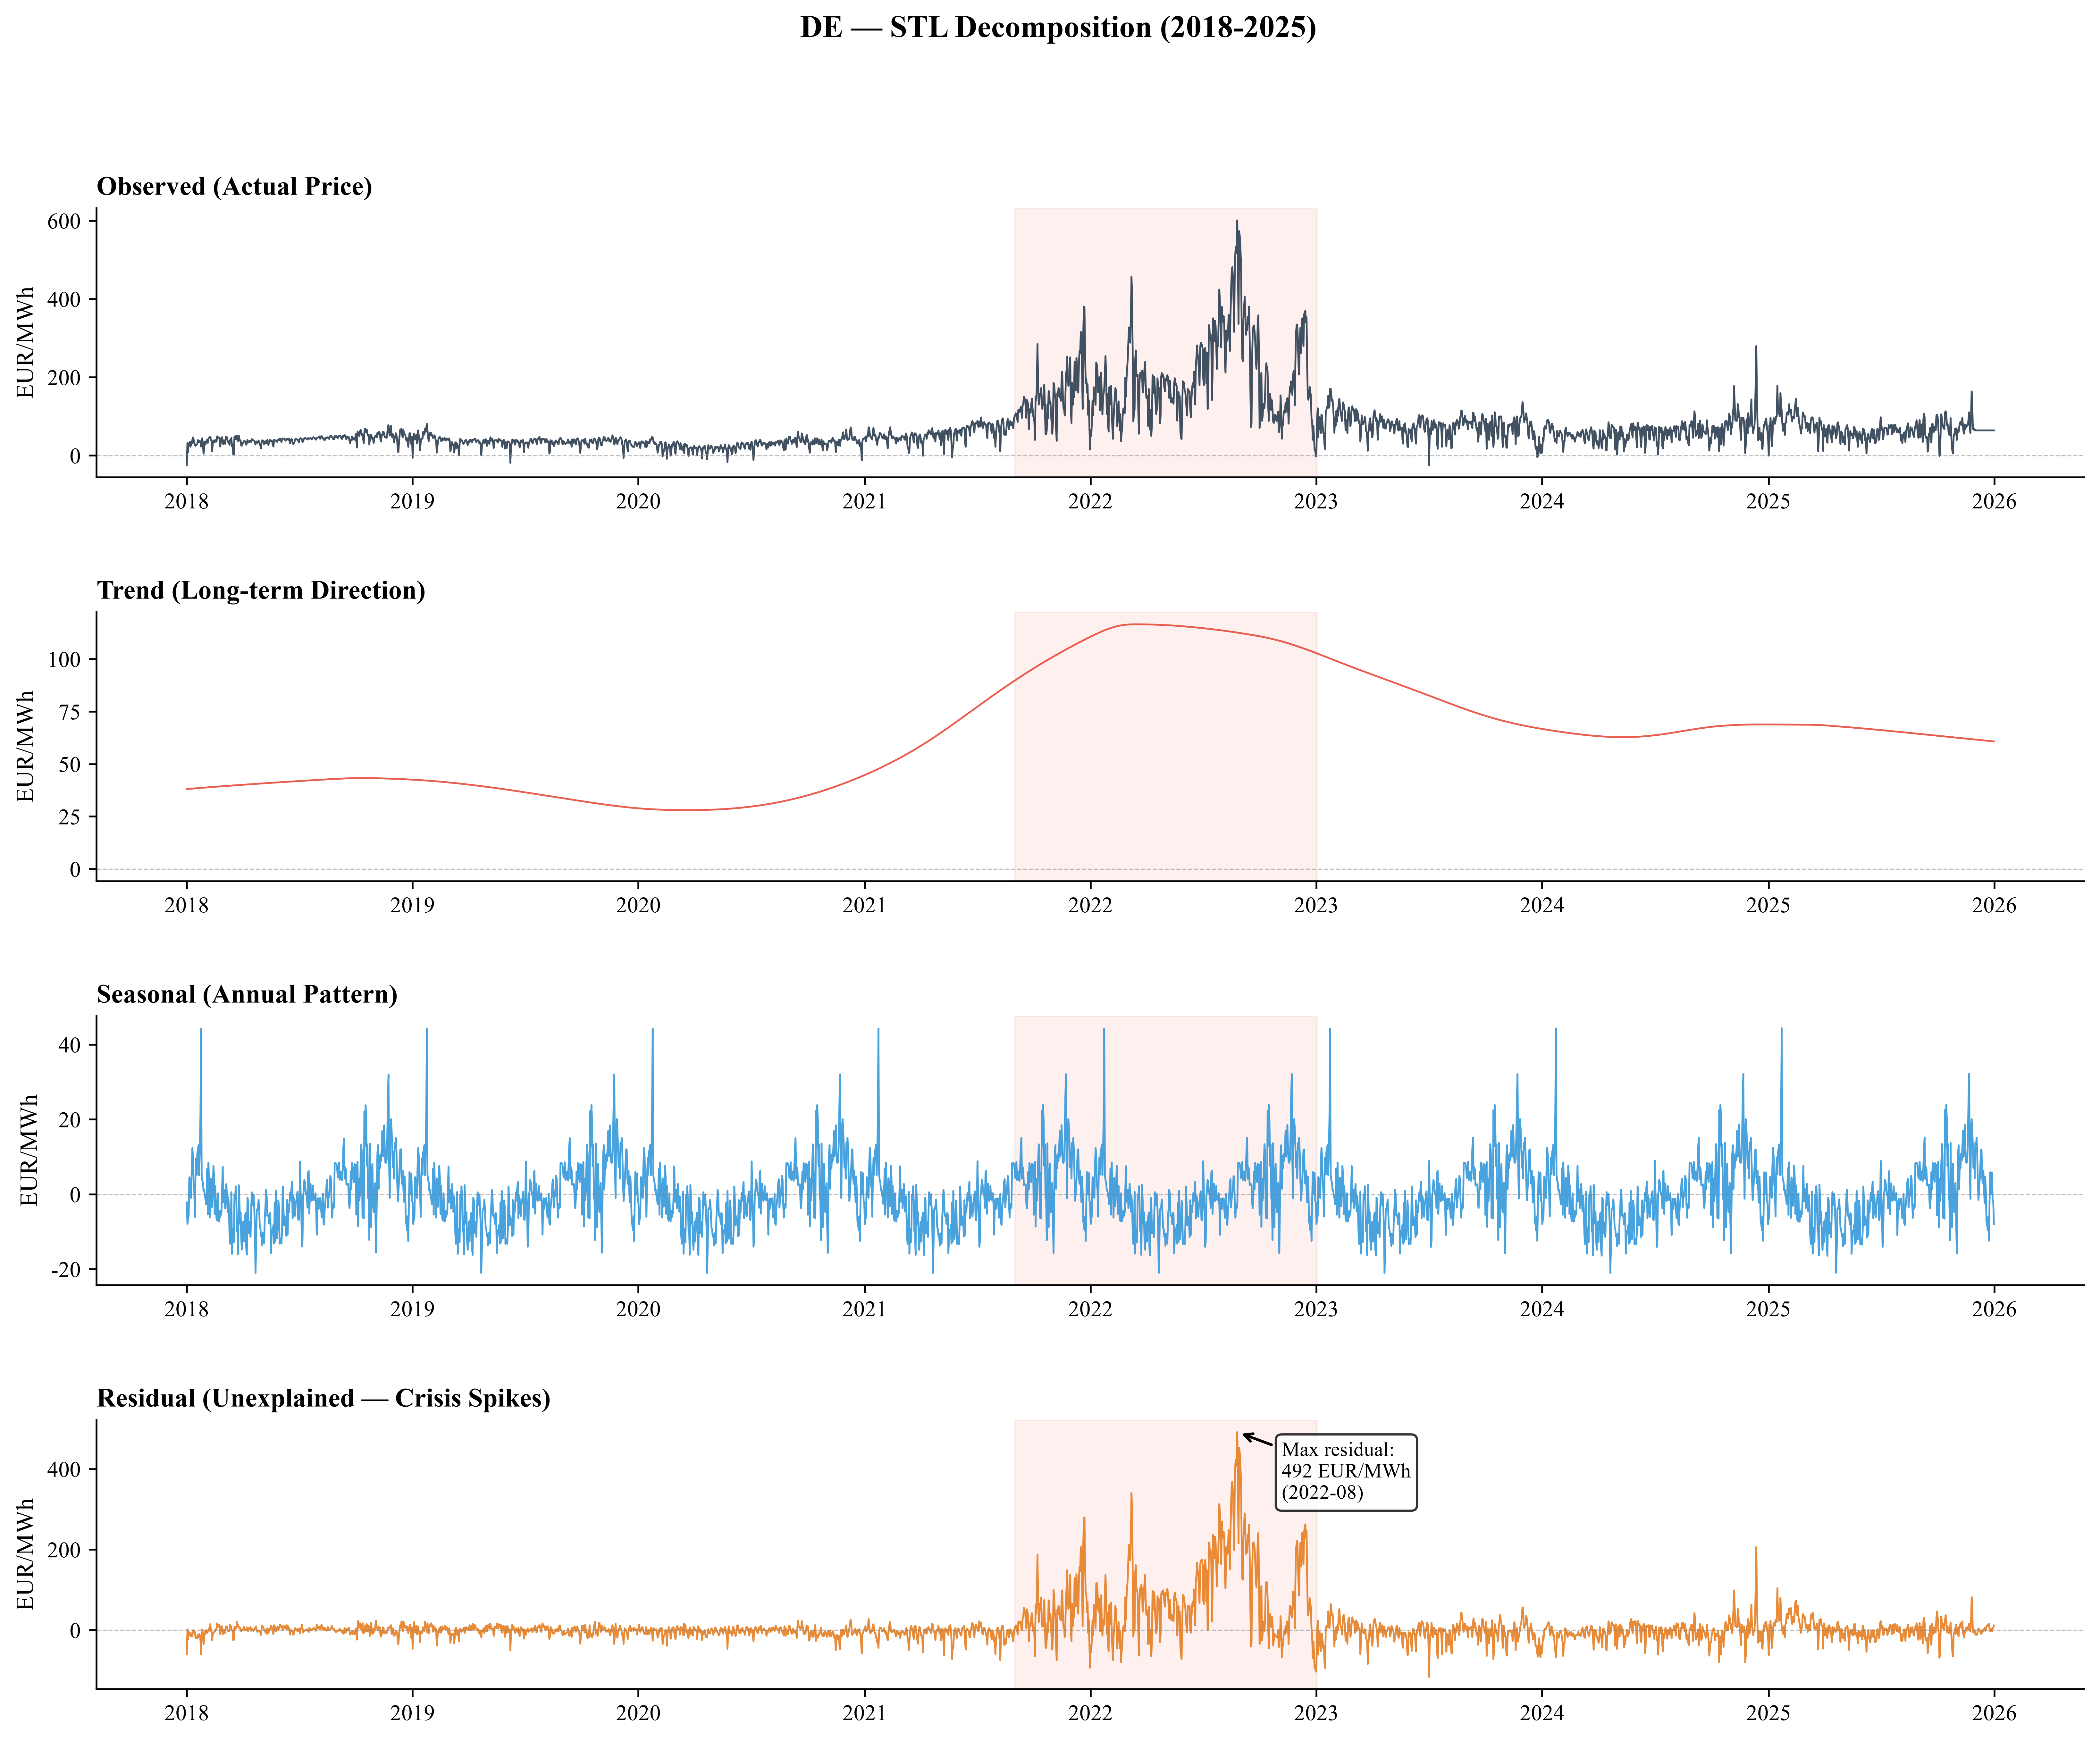
\includegraphics{figures/methodology/DE_stl_annual.png}
  \end{adjustbox}
  \captionof{figure}{Kết quả phân rã chuỗi thời gian STL giá điện thực tế tại Đức (DE)}
  \label{fig:de_stl}
  \vspace{0.08cm}
  \parbox{0.9\textwidth}{\small \textit{Ghi chú:} Đức được chọn làm ví dụ đại diện do có cấu trúc nguồn phát đa dạng nhất. Biểu đồ gồm 3 thành phần phân rã: xu hướng dài hạn ($T_t$), mùa vụ ($S_t$) và phần dư ($R_t$) bên cạnh chuỗi gốc ($P_t$). Vùng đổ bóng hồng biểu thị giai đoạn khủng hoảng năng lượng châu Âu (9/2021--1/2023).}
  \end{minipage}
\end{strip}

Hình~\ref{fig:umap_clusters} trình bày không gian nhúng UMAP 2D tại Đức (DE) làm quốc gia đại diện, trong đó mỗi điểm dữ liệu được tô màu theo thể chế ($R_0, R_1, \ldots$). Sự tách biệt không gian rõ ràng giữa cụm khủng hoảng 2022 và các thể chế thời bình cung cấp ranh giới phân loại phi tuyến khách quan cho mô hình hóa XGBoost ở Mục~\ref{subsec:shap_evolution}.

Để trả lời câu hỏi \textit{"Ngưỡng nào thì thị trường chuyển từ trạng thái bình thường sang khủng hoảng?"}, phân tích tương tác phi tuyến chỉ ra một ranh giới chuyển dịch nhất quán. Cụ thể, khi giá khí TTF vượt ngưỡng khoảng 60--80 EUR/MWh đồng thời tải trọng còn lại vượt ngưỡng 60--70\% công suất đỉnh hệ thống, thị trường chuyển dịch từ thể chế vận hành nền sang thể chế giá bùng nổ cận biên. Sự phân định này được bảo đảm tính hợp lệ tối ưu nhờ chỉ số mật độ DBCV, giữ cho ranh giới phi tuyến trung thực với thực tế mà không bị nhiễu cục bộ làm sai lệch.

Về mặt học thuật, nhãn thể chế HDBSCAN loại bỏ hiện tượng trung bình hóa sai số OLS toàn cục, giúp cây quyết định học được luật chia nhánh riêng biệt.

\begin{figure}[h!]
  \centering
  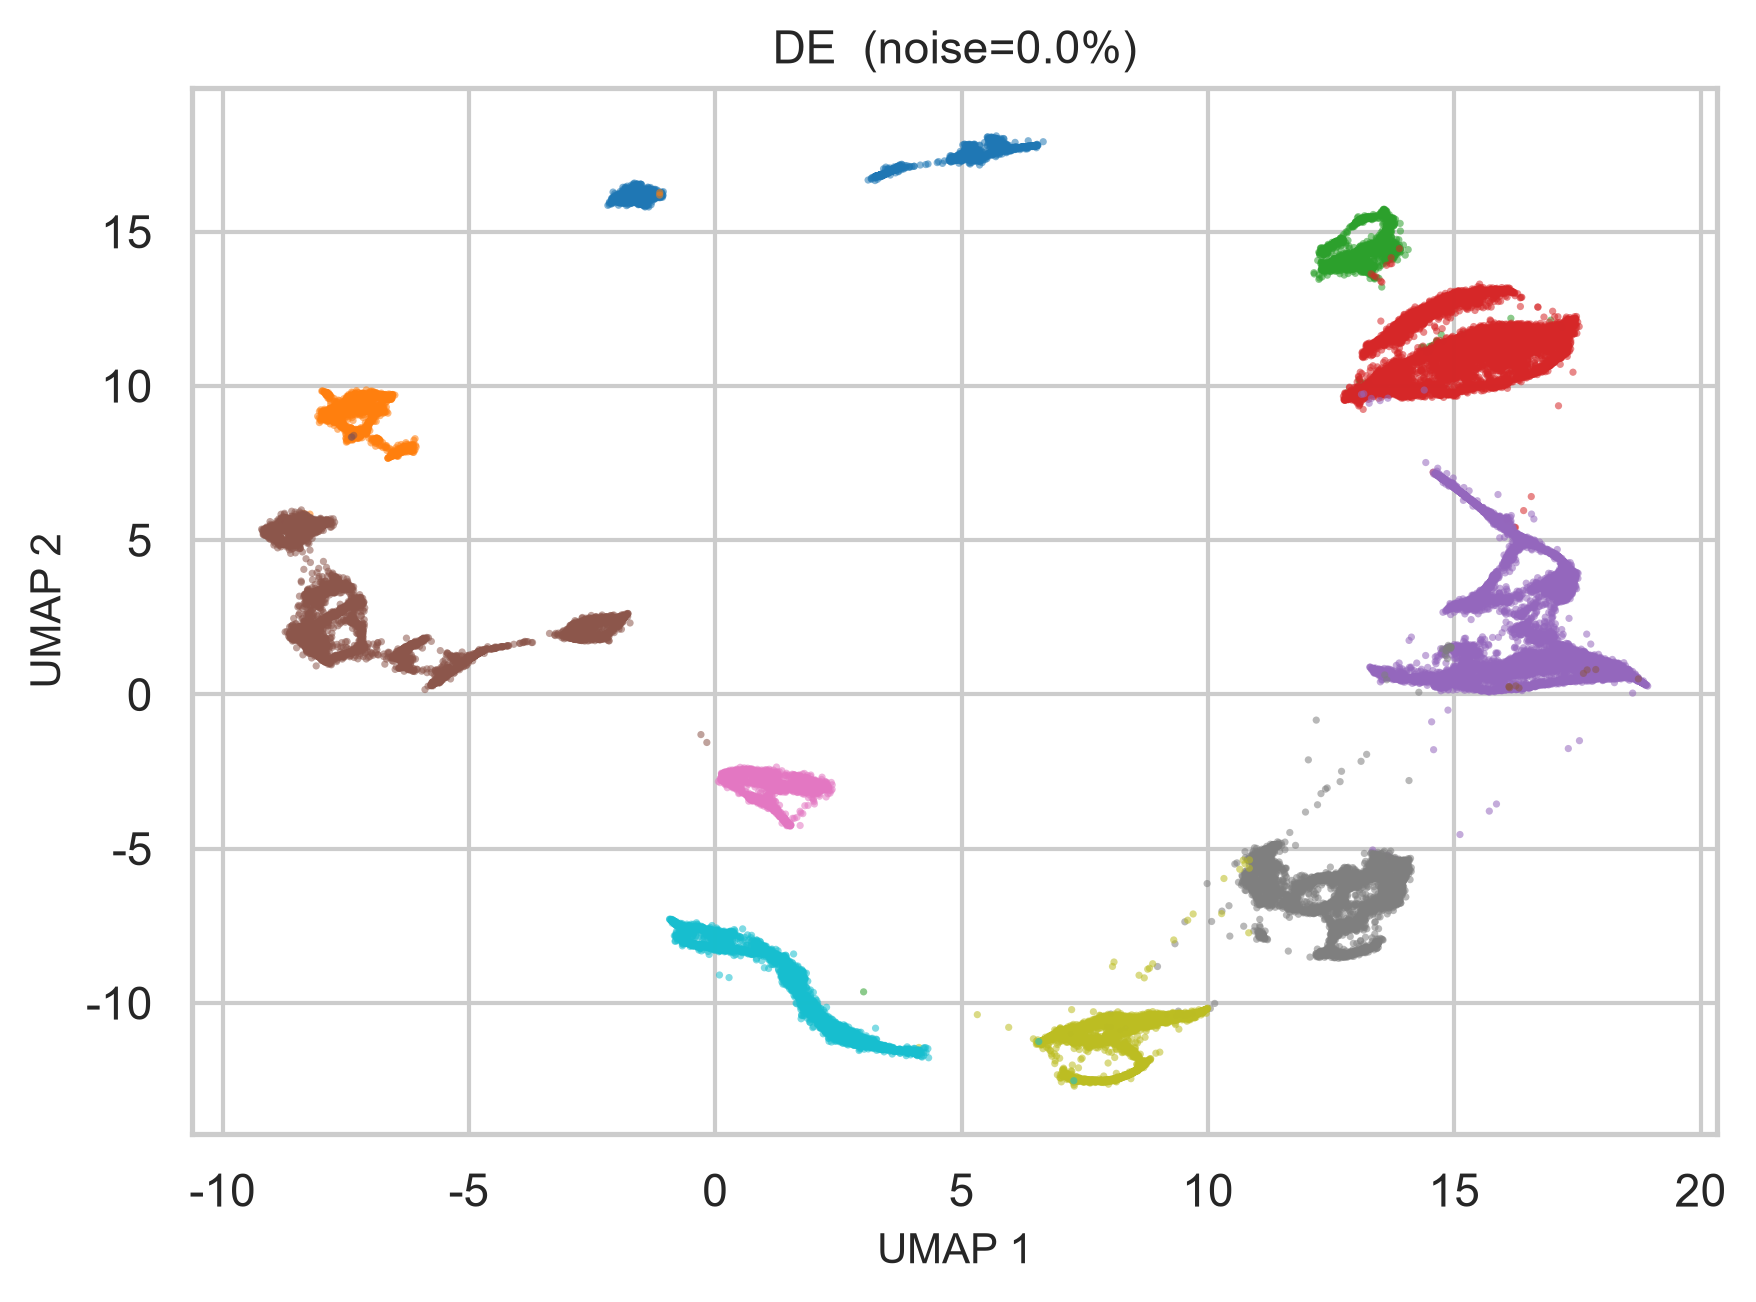
\includegraphics[width=\columnwidth]{figures/results/umap_hdbscan_regime_clusters.png}
  \caption{Không gian nhúng UMAP 2D của phân cụm HDBSCAN tại Đức (DE)}
  \label{fig:umap_clusters}
  \vspace{0.05cm}
  \parbox{\columnwidth}{\small \textit{Ghi chú:} Mỗi màu tương ứng một thể chế thị trường ($R_0$--$R_9$); điểm xám là nhiễu (Noise).}
\end{figure}

\subsection{Đánh giá hiệu suất mô hình qua các cửa sổ Walk-Forward}
\label{subsec:shap_evolution}

Để kiểm chứng năng lực thích ứng của mô hình trước các thay đổi cấu trúc ngoại sinh, Bảng~\ref{tab:wf_r2} trình bày chỉ số độ chính xác $R^2$ thực nghiệm của XGBoost qua sáu cửa sổ kiểm định Walk-Forward Expanding Window ($W_1$ đến $W_6$).

\begin{table}[h!]
\caption{Cấu hình HDBSCAN tối ưu và chỉ số đánh giá theo quốc gia}
\label{tab:hdbscan_results}
\centering
\small
\begin{tabular}{@{}l c c c c@{}}
\toprule
Quốc gia & mcs & ms & Số cụm & Nhiễu (Noise) \\
\midrule
Đức (DE) & 300 & 50 & 10 & 0,0\% \\
Đan Mạch (DK) & 500 & 10 & 7 & 0,0\% \\
Tây Ban Nha (ES) & 500 & 10 & 5 & 6,3\% \\
Pháp (FR) & 400 & 10 & 8 & 4,6\% \\
Ý (IT) & 500 & 10 & 5 & 4,1\% \\
Ba Lan (PL) & 400 & 10 & 7 & 4,3\% \\
\bottomrule
\end{tabular}
\vspace{0.15cm}
\begin{minipage}{\columnwidth}
\small\textit{Ghi chú:} mcs và ms lần lượt là các tham số min\_cluster\_size và min\_samples. Tỷ lệ nhiễu là tỷ lệ quan sát không thuộc cụm thể chế xác định, được tối ưu dựa trên chỉ số mật độ DBCV.
\end{minipage}
\end{table}

\begin{table}[h!]
  \centering
  \footnotesize
  \setlength{\tabcolsep}{3.5pt}
  \caption{Chỉ số $R^2$ của mô hình XGBoost cấu hình $C_1$ qua sáu cửa sổ kiểm định Walk-Forward}
  \label{tab:wf_r2}
  \vspace{0.1cm}
  \begin{tabular*}{\columnwidth}{@{\extracolsep{\fill}}lcccccc@{}}
    \toprule
    \textbf{Quốc gia} & $\mathbf{W_1}$ & $\mathbf{W_2}$ & $\mathbf{W_3}$ & $\mathbf{W_4}$ & $\mathbf{W_5}$ & $\mathbf{W_6}$ \\
    \midrule
    Đức (DE)         & 0,626 & -0,695 & -2,187 & 0,533 & 0,598 & 0,528 \\
    Đan Mạch (DK)    & 0,072 & -0,172 & -1,477 &  0,366 & 0,326 & 0,289 \\
    Tây Ban Nha (ES) & 0,573 & -0,615 & -12,503 &  -0,435 & 0,406 & 0,356 \\
    Pháp (FR)        & 0,016 & -0,354 & -3,079 &  0,414 & -0,002 & 0,505 \\
    Ý (IT)           & 0,117 & -0,470 & -4,570 &  0,591 & 0,411 & -0,852 \\
    Ba Lan (PL)      & 0,084 & -0,138 & -2,645 & -0,008 & 0,231 & 0,282 \\
    \bottomrule
  \end{tabular*}
  \vspace{0.1cm}
  \begin{minipage}{\columnwidth}
    \footnotesize \textit{Ghi chú:} Cửa sổ $W_3$ tương ứng với năm khủng hoảng 2022 ($R^2 < 0$). $C_1$ = 6 biến vĩ mô không có nhãn thể chế.
  \end{minipage}
\end{table}

Kết quả thực nghiệm cho thấy mô hình $C_1$ (sáu biến vĩ mô) đạt $R^2$ tốt tại các cửa sổ bình thường, dao động từ 0,02 đến 0,63 ($W_1, W_4, W_5, W_6$), khẳng định các biến nhân quả vĩ mô giải thích được phần lớn biến động giá điện. Tại cửa sổ $W_3$ (năm 2022), $R^2$ sụt giảm đồng loạt xuống mức âm sâu trên toàn bộ sáu quốc gia (thấp nhất là Tây Ban Nha với $-12{,}50$); về mặt thống kê, $R^2 < 0$ có nghĩa là mô hình dự báo còn kém hơn cả đường cơ sở dự báo bằng giá trị trung bình, tức là mô hình không còn bất kỳ sức mạnh giải thích nào trong cửa sổ này. Đây là bằng chứng thực nghiệm rõ nét về hiện tượng dịch chuyển phân phối (distribution shift): khủng hoảng năm 2022 tạo ra một chế độ giá hoàn toàn ngoài vùng lịch sử huấn luyện, vượt khỏi khả năng ngoại suy của mô hình cây quyết định. Sự phục hồi $R^2$ sang cửa sổ $W_4$ (2023) khi dữ liệu khủng hoảng được đưa vào tập huấn luyện xác nhận nhận định này.

\subsection{Thảo luận định lượng SHAP về cơ cấu chi phí phát điện cận biên}

Để giải thích cơ chế tác động biên của từng nhân tố tới giá điện bán buôn, Bảng~\ref{tab:shap_top5} trình bày Top~5 đặc trưng có đóng góp tuyệt đối trung bình $|\text{SHAP}|$ cao nhất tại sáu thị trường theo cấu hình $C_1$.

\begin{table}[h!]
  \centering
  \footnotesize
  \setlength{\tabcolsep}{4pt}
  \caption{Top 5 đặc trưng quan trọng nhất theo định lượng SHAP tuyệt đối trung bình (cấu hình $C_1$)}
  \label{tab:shap_top5}
  \vspace{0.1cm}
  \begin{tabular*}{\columnwidth}{@{\extracolsep{\fill}}llrr@{}}
    \toprule
    \textbf{Q.Gia} & \textbf{Đặc trưng} & \textbf{$|\mathbf{SHAP}|$} & \textbf{T\%} \\
    \midrule
    \textbf{DE} & Residual\_Load     & 20,31 & 55,5\% \\
                & Coal\_Price        &  7,89 & 21,6\% \\
                & TTF\_Gas\_Price    &  3,43 &  9,4\% \\
                & Brent\_Oil\_Price  &  2,17 &  5,9\% \\
                & EU\_ETS\_Price     &  1,63 &  4,5\% \\
    \midrule
    \textbf{DK} & Residual\_Load     & 14,59 & 50,1\% \\
                & Coal\_Price        &  5,96 & 20,4\% \\
                & EU\_ETS\_Price     &  3,05 & 10,5\% \\
                & TTF\_Gas\_Price    &  3,05 & 10,5\% \\
                & Brent\_Oil\_Price  &  1,61 &  5,5\% \\
    \midrule
    \textbf{ES} & Residual\_Load     & 13,75 & 48,4\% \\
                & TTF\_Gas\_Price    &  8,88 & 31,2\% \\
                & Coal\_Price        &  2,53 &  8,9\% \\
                & Brent\_Oil\_Price  &  2,04 &  7,2\% \\
                & EU\_ETS\_Price     &  0,89 &  3,1\% \\
    \midrule
    \textbf{FR} & Residual\_Load     & 17,66 & 49,0\% \\
                & Coal\_Price        &  8,51 & 23,6\% \\
                & TTF\_Gas\_Price    &  5,92 & 16,4\% \\
                & Brent\_Oil\_Price  &  2,78 &  7,7\% \\
                & EU\_Gas\_Storage   &  0,61 &  1,7\% \\
    \midrule
    \textbf{IT} & Residual\_Load     & 12,23 & 38,0\% \\
                & Coal\_Price        & 11,52 & 35,8\% \\
                & TTF\_Gas\_Price    &  3,93 & 12,2\% \\
                & Brent\_Oil\_Price  &  2,31 &  7,2\% \\
                & EU\_Gas\_Storage   &  1,09 &  3,4\% \\
    \midrule
    \textbf{PL} & Residual\_Load     & 11,97 & 44,3\% \\
                & Coal\_Price        &  5,84 & 21,6\% \\
                & TTF\_Gas\_Price    &  5,59 & 20,7\% \\
                & Brent\_Oil\_Price  &  1,48 &  5,5\% \\
                & EU\_ETS\_Price     &  1,43 &  5,3\% \\
    \bottomrule
  \end{tabular*}
  \vspace{0.1cm}
  \begin{minipage}{\columnwidth}
    \footnotesize \textit{Ghi chú:} T\% = tỷ trọng trong tổng \textit{mean}~$|\text{SHAP}|$ của $C_1$. EU\_Gas\_Storage = EU\_Gas\_Storage\_Anomaly.
  \end{minipage}
\end{table}

Bảng~\ref{tab:shap_top5} chỉ ra sự phân hóa thể chế rất rõ ràng giữa các quốc gia châu Âu:
\begin{enumerate}
  \item \textbf{Vai trò chủ đạo của Tải trọng còn lại:} Tại cả sáu thị trường, \textit{Residual\_Load} luôn giữ vị trí số một với tỷ trọng từ 38,0\% (Ý) đến 55,5\% (Đức), khẳng định nguyên lý trật tự ưu tiên huy động Merit Order.
  \item \textbf{Than vượt trội khí tại 5/6 quốc gia:} \textit{Coal\_Price} dẫn trước \textit{TTF\_Gas\_Price} tại Đức, Đan Mạch, Pháp, Ý và Ba Lan, chứng tỏ than vẫn là nhiên liệu cận biên quyết định giá tại phần lớn thị trường. Ngoại lệ duy nhất là Tây Ban Nha, nơi cơ chế áp trần giá khí đốt phát điện (Iberian Exception -- ngoại lệ bán đảo Iberia) đẩy TTF lên hàng hai (31,2\%).
  \item \textbf{Độ nhạy TTF theo đặc thù thị trường:} Tại Ba Lan, TTF đạt 20,7\% phản ánh sự chuyển dịch dần khỏi nền than. Tại Ý (IT), tỷ lệ Than (35,8\%) áp đảo TTF (12,2\%), cho thấy than đóng vai trò cận biên thực sự chủ đạo trong giai đoạn nghiên cứu do hiện tượng chuyển dịch nhiên liệu (fuel switching) khi giá khí TTF tăng cực mạnh năm 2022.
  \item \textbf{Vai trò kết nối của giá dầu thô Brent:} \textit{Brent\_Oil\_Price} xuất hiện nhất quán trong Top~5 tại cả sáu thị trường (5,5--7,7\%), hoạt động như một biến nhân quả trung gian (mediating variable) kết nối thị trường năng lượng toàn cầu với thị trường điện châu Âu thông qua kênh định giá hợp đồng khí đốt dài hạn có chỉ số dầu mỏ.
\end{enumerate}

Những phát hiện định lượng này cung cấp cơ sở vững chắc cho các nhà hoạch định chính sách trong việc thiết kế các cơ chế bình ổn giá phù hợp với đặc thù cấu trúc nguồn phát của từng quốc gia. Cụ thể, danh mục Top~5 SHAP theo quốc gia có thể được trực tiếp sử dụng như một \textit{bảng điều khiển chỉ số cảnh báo sớm} (early-warning dashboard): khi các biến dẫn đầu (Residual\_Load, TTF hoặc Coal tùy quốc gia) đồng loạt vượt ngưỡng lịch sử, xác suất chuyển dịch thể chế sang vùng giá cực đoan tăng lên đáng kể.


% ============================================================


% ============================================================
% sections/conclusion.tex
% Section 4: KẾT LUẬN

\section{Kết luận}

Nghiên cứu này đã đề xuất và kiểm chứng thực nghiệm thành công một quy trình khai phá dữ liệu bốn giai đoạn nhằm phát hiện các thể chế vận hành phi tuyến của thị trường điện bán buôn và giải thích cơ chế hình thành giá bán buôn tại sáu quốc gia châu Âu giai đoạn 2018--2025. Các kết luận khoa học chính thu được bao gồm:

\begin{enumerate}
  \item Bản chất phi mùa vụ của cuộc khủng hoảng: Kết quả phân rã chuỗi thời gian STL chỉ ra rằng cuộc khủng hoảng năng lượng năm 2022 nằm hoàn toàn trong thành phần phần dư ($R_t$), không chịu ảnh hưởng bởi các yếu tố xu hướng dài hạn hay tính mùa vụ thông thường. Điều này khẳng định sự cần thiết phải tích hợp các biến đặc trưng nhân quả bên ngoài như giá khí đốt và độ lệch trữ lượng kho để giải thích các đột biến giá.
  \item Cơ sở nhân quả vững chắc: Các kiểm định nhân quả Granger đã xác nhận tính đúng đắn của chuỗi liên kết Merit Order đề xuất trong đồ thị DAG hướng từ đặc trưng vật lý của hệ thống và giá nhiên liệu đến giá điện bán buôn thực tế.
  \item Giá trị diễn giải của thể chế thị trường: Việc kết hợp UMAP và phân cụm mật độ HDBSCAN đã nhận diện thành công từ năm đến mười thể chế thị trường phi tham số trên mỗi quốc gia. Kiểm định thực nghiệm cho thấy phân cụm thể chế không cải thiện độ chính xác dự báo một cách nhất quán ($\Delta R^2 = +0,012$): XGBoost đã nội tại hóa cấu trúc thể chế từ sáu biến đầu vào. Tuy nhiên, nhãn thể chế cung cấp \textit{giá trị diễn giải}: công cụ giám sát trạng thái thị trường có thể đọc được (interpretable) cho các nhà điều tiết.
  \item Bằng chứng thực nghiệm về dịch chuyển phân phối: Việc sụt giảm chỉ số $R^2$ xuống giá trị rất âm vào năm 2022 ($W_3$) và sự hồi phục mạnh mẽ vào năm 2023 ($W_4$) khi dữ liệu khủng hoảng được huấn luyện là bằng chứng thực nghiệm rõ nét nhất chứng minh hiện tượng dịch chuyển phân phối dữ liệu (distribution shift) do mô hình cây quyết định không có khả năng ngoại suy nằm ngoài vùng lịch sử.
  \item Giá trị thực tiễn của ranh giới khủng hoảng: Nghiên cứu đã chỉ ra ranh giới khủng hoảng phi tuyến trong không gian sáu biến trạng thái ($C_1$: TTF, Coal, EU ETS, Brent, Residual Load, Storage): khi $\text{Residual\_Load} > 65\%$ và $\text{TTF} > 60\text{--}80$ EUR/MWh, thị trường chuyển sang thể chế giá bùng nổ cận biên.
\end{enumerate}

Hàm ý chính sách: Kết quả nghiên cứu cung cấp một công cụ giám sát rủi ro thực tế cho các cơ quan điều tiết năng lượng và nhà điều hành hệ thống truyền tải (TSO). Bằng cách liên tục giám sát vị trí trạng thái hệ thống trong không gian sáu biến ($C_1$: TTF, Coal, EU ETS, Brent, Residual Load, Storage Anomaly) so với ranh giới khủng hoảng thực nghiệm được xác định, các bên liên quan có thể đưa ra các cảnh báo sớm và biện pháp can thiệp thị trường kịp thời nhằm ngăn chặn các hành vi tăng giá cực đoan.

% ============================================================
% ACKNOWLEDGMENTS (unnumbered)
% ============================================================
\section*{LỜI CẢM ƠN}

Nghiên cứu này được hỗ trợ bởi các nguồn dữ liệu công khai từ EMBER, ENTSO-E, Gas Infrastructure Europe (GIE) và Ngân hàng Thế giới. Tác giả chân thành cảm ơn các nhà phản biện và đồng nghiệp đã cung cấp các ý kiến quý báu để hoàn thiện phương pháp luận nghiên cứu.

% ============================================================

% ============================================================
% REFERENCES (unnumbered)
% ============================================================
\section*{TÀI LIỆU THAM KHẢO}
\printbibliography[heading=none]

\end{document}
